%%%%%%%%%%%%%%%%%%%%%%%%%%%%%%%%%%%%%%%%%%%%%%%%%%%%%%
%
% This file defines the style for your report.
%
% Just run "sh compiletex.sh" to compile
% 
%%%%%%%%%%%%%%%%%%%%%%%%%%%%%%%%%%%%%%%%%%%%%%%%%%%%%%

\documentclass[10pt,  english, makeidx, a4paper, titlepage, oneside]{book}
\usepackage{babel}
\usepackage{fancyhdr}
\usepackage{makeidx}
\usepackage{titlesec}
\usepackage{listings}
\usepackage{booktabs}
\usepackage{hyperref}

\newenvironment{listato}{\footnotesize}{\normalsize }

\textwidth 15.5cm
\textheight 23cm
\topmargin -1cm
\oddsidemargin -0.5cm
\linespread{1.1}

\pagestyle{fancy}
\lhead{}
\chead{Cybersecurity for Embedded Systems}
\lfoot{}
\cfoot{}
\rfoot{}
\rhead{\thepage}

\usepackage{graphicx}
\usepackage{amsmath}
\usepackage{amsfonts}
\usepackage{amsthm}
\usepackage{amssymb}
\usepackage{graphicx}
\usepackage{caption}
\usepackage{float}
\usepackage{amsmath}
\usepackage{amssymb}
\usepackage{amsfonts}
\usepackage{amsthm}
\usepackage{empheq}
\usepackage{verbatim}
\usepackage{fancyvrb}
\usepackage{xcolor}

\titleformat{\chapter}[display]
{\normalfont\Large\filcenter\sffamily}
{\titlerule[0.5pt]%
\vspace{1pt}
\titlerule
\vspace{1pc}
\LARGE\MakeUppercase{\chaptertitlename} \thechapter
}
{1pc}
{\titlerule
\vspace{1pc}
\Huge}

\makeindex

\begin{document}

\frontmatter
\begin{titlepage}
\vspace{0cm}
\centerline{

\includegraphics[width=6cm]{./logopolitonuovo}} 
\vspace{0.5cm}
\centerline{\LARGE Politecnico di Torino}
\vspace{2.5cm}
\centerline{\huge Cybersecurity for Embedded Systems}
\vspace{0.25cm}
\centerline{\huge 01UDNOV}
\vspace{1cm}
\centerline{\Large Master's Degree in Computer Engineering}
\vspace{2.5cm}
\centerline{\Huge Project Title}
\bigskip
\centerline{\huge Project Report}
\vspace{2cm}
\vfill
\begin{minipage}{6.5cm} % modify this width in order to keep everything on the same line
\Large{Candidates:\\
Name Surname (student ID)\\
Name Surname (student ID)\\
Name Surname (student ID)}
\end{minipage}
\hfill
\begin{minipage}{4.4cm}
\Large{Referee: \\
Prof. Paolo Prinetto}
\end{minipage}
\end{titlepage}

\tableofcontents
\listoffigures % REMOVE THIS IF THERE ARE NO PICTURES
\listoftables % REMOVE THIS IF THERE ARE NO TABLES

\mainmatter
    
% HERE IS WHERE YOU INCLUDE YOUR CHAPTERS

\chapter*{Abstract}
%This is the space reserved for the abstract of your report. The abstract is a summary of the report, so it is a good idea to write after all other chapters. The abstract for a thesis at PoliTO must be shorter than 3500 chars, try to be compliant with this rule (no problem for an abstract that is a lot shorter than 3500 chars, since this is not a thesis).
%Use short sentences, do not use over-complicated words. Try to be as clear as possible, do not make logical leaps in the text. Read your abstract several times and check if there is a logical connection from the beginning to the end. The abstract is supposed to draw the attention of the reader, your goal is to write an abstract that makes the reader wanting to read the entire report. Do not go too far into details; if you want to provide data, do it, but express it in a simple way (e.g., a single percentage in a sentence): do not bore the reader with data that he or she cannot understand yet. Organize the abstract into paragraphs: the paragraphs are always 3 to 5 lines long. In \LaTeX source file, go new line twice to start a new paragraph in the PDF. Do not use $\\$ to go new line, just press Enter. In the PDF, there will be no gap line, but the text will go new line and a Tab will be inserted. This is the correct way to indent a paragraph, please do not change it. Do not put words in \textbf{bold} here: for emphasis, use \emph{italic}. Do not use citations here: they are not allowed in the abstract. Footnotes and links are not allowed as well. DO NOT EVER USE ENGLISH SHORT FORMS (i.e., isn't, aren't, don't, etc.).
%Take a look at the following links about how to write an Abstract:
%\begin{itemize}
%\item \url{https://writing.wisc.edu/handbook/assignments/writing-an-abstract-for-your-research-paper/}
%\item \url{https://www.anu.edu.au/students/academic-skills/research-writing/journal-article-writing/writing-an-abstract}
%\end{itemize}
%Search on Google if you need more info.

Physically Unclonable Functions (PUFs) have gained significant attention in the hardware security domain, due to their ability to generate unique identifiers
from physical variations in hardware components, which helps in the authentication and key generation domains. This report provides a comprehensive description
of a particular PUF design, called CamPUF, which is based on CMOS image sensors.

Inherent physical processes happening in image sensors are exploited, such as Fixed Pattern Noise and, in particular, one of its sources: the Dark Signal Non-Uniformity (DSNU).
DSNU can be extracted by dark digital images, which means that a fingerprint based on this noise is harder to extract from illuminated images, where PRNU and other type of noises are prevalent.
This design also includes an efficient and reliable key generation algorithm and a computationally light device authentication mechanism.

A complete implementation of the CamPUF is provided, along with a high-level view of the solution and an explanation of the theory which is at the basis of this design.
This document will show a comprehensive description, a complete testing procedure, along with the steps to replicate it, and an overview of the results, which
will highlight the strengths and the reliability of this PUF design. At last, we also present an \textit{attack mitigation} section, to show the security against
possible counterfeiting measures.






\chapter{Generic Chapter}
This is a generic chapter of your thesis. Remember to put ANY chapter in a different source file (including introduction and all the others).

For the purpose of this guide, the main \LaTeX constructs and how to use them will be explained here. Other thematic chapters will follow, i.e., which will trace the chapters that should be present in your thesis. Delete this generic chapter once you have learned this contents.

You can write in italic \emph{like this}, you can write in bold \textbf{like this}, or you can write using colors \textcolor{cyan}{like this}.

This is an \emph{itemize}, where you can put a list of items, like this:
\begin{itemize}
	\item item number 1
	\item item number 2
\end{itemize}

This is an \emph{enumerate}, where you can put a list of items with numbers, like this:
\begin{enumerate}
	\item item number 1
	\item item number 2
\end{enumerate}

You can cite references like this: \cite{texbook} \cite{lamport94}, by using the \lstinline{\cite} directive. You have to copy within \lstinline{\cite} brackets the label of the entry that you have in the BibTeX file (\texttt{.bib}). The \texttt{.bib} file of this thesis is \texttt{mybib.bib}. he command \lstinline{\addbibresource} at the top of this main file indicates what BibTeX file you are referring to.

As an example, this is a BibTeX entry:

\begin{verbatim}
@inproceedings{urias2018cyber,
  title={Cyber Range Infrastructure Limitations and Needs of Tomorrow: A Position Paper},
  author={Urias, Vincent E and Stout, William MS and Van Leeuwen, Brian and Lin, Han},
  booktitle={2018 International Carnahan Conference on Security Technology (ICCST)},
  pages={1--5},
  year={2018},
  organization={IEEE}
}
\end{verbatim}

For every online paper that you may read on online libraries, you can download its BibTeX entry. For example:
\begin{enumerate}
	\item For IEEE Xplore, click on the paper name, then click on ``Cite This'', ``BibTeX'', and you can find the entry;
	\item For Google Scholar, click on the ``Cite'' voice under the paper name, then click ``BibTeX'', and you can find the entry.
\end{enumerate}

Just copy and paste such an entry in the .bib file. If you find a paper on Scholar that is nevertheless published by IEEE, by convention you should take the entry from the IEEE website and not from Scholar. To do this, just click on the title of the paper. This will redirect you to the resource page on IEEE Xplore. Once here, follow instructions at point 1.

When you compile, a correct number will automatically be assigned to the citation in the text, and the complete entry will appear at the bottom of the document, in the ``Bibliography'' chapter.

If you need to cite a generic online resource, which does not necessarily correspond to a scientific paper, use the \lstinline{@misc} entry in the \texttt{.bib} file. A \lstinline{@misc} entry looks like this:

\begin{verbatim}
@misc{nist2018,
    author = "{NIST}",
    title = "Cyber Ranges",
    year = "2018",
    howpublished = "\url{https://www.nist.gov/system/files/documents/2018/02/13/cyber_ranges.pdf}",
    note = "[Online; Accessed 2019, 28 November]"
  }
\end{verbatim}

You have to manually create this entry from scratch and manually type these fields. Remember not to forget any of these fields. You can choose the label with which to refer to the resource. The title of the website (which you can see at the top of the tab of your browser showing the page) can be used as the title of the resource.

In general, enter a citation of this type for sites only when there are data, phrases, or images that you intend to report. Instead, if you want to cite names of software or hardware devices, prefer the use of the \lstinline{\footnote}, in which you will only have to specify the URL of the item.

Remember that citations, both in the text and in the image captions, usually go to the end of a sentence, before the fullstop, as in this case \cite{vykopal2017kypo}. In case of long periods, they can also be placed before other detachment signs, such as commas or semicolons, or colons if they precede a list, itemized or enumerated. An exemption is allowed in the event that the name of research projects, described in some scientific resource, is being introduced, as in this case:

\begin{center}
	Cybertropolis \cite{deckard2018cybertropolis} is described in a very good paper by Gary Deckard.
\end{center}

Remember to put citations very often to justify your claims, especially when you report data or results. Just consider them as a justification of what you, in an original way, are writing. Citations are not needed to have permission to copy and paste sentences from online resources, which should NEVER be done - always try to rephrase the concept with your words.

\begin{figure}[h!]
	\vspace{0.5cm}
	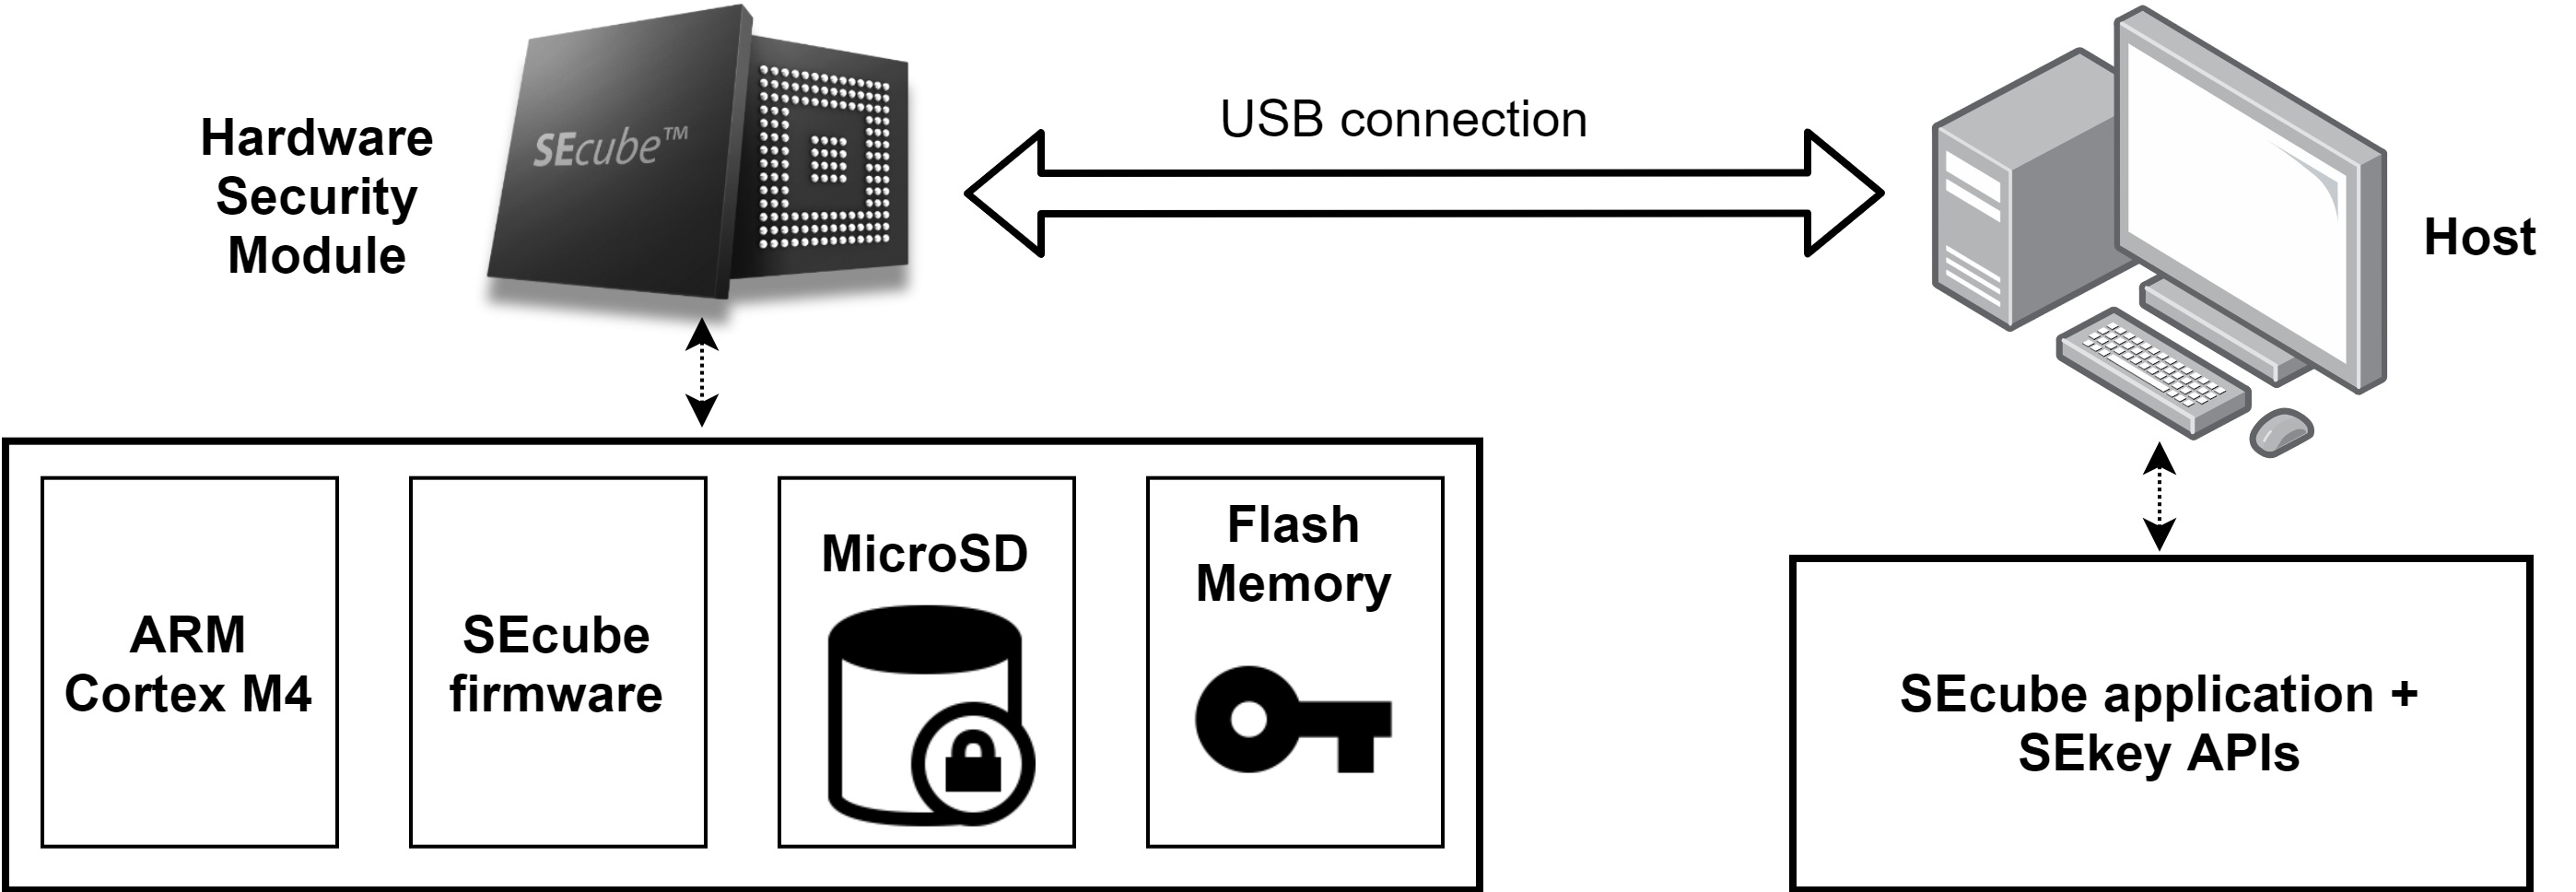
\includegraphics[width=\textwidth]{images/simplearch.jpg}
	\caption{This is the image \emph{caption}.}
	\label{fig:generalschema} % This is the image label, with which you can refer to the image in any document location.
\end{figure}

This is an image example. Images must ALWAYS be understandable: never introduce images that have text smaller than the text in your document. If you create the images yourself, try not to make them clash too much with the style of your document, and use the same font as this thesis.
If they are not images of your own creation, you MUST reference them. In the caption of the image, you need to insert a citation to the resource from which you took the image, at the end of the caption sentence, before the fullstop.
Each image you enter MUST be referenced in the text, using a formula similar to this:

\begin{center}
	Figure \ref{fig:generalschema} describes the architecture of the system.
\end{center}

You can refer to the image using \lstinline{\ref} followed by the image label, that you put in the \lstinline{\label} entry of the figure. Remember to use the word Figure with a capital F.

Remember that the more your text is adorned with figures, the more understandable, appreciable and readable it becomes.

\section{Section title}\label{examplesection}
This is a section under a chapter. The number of sections also contributes to greater readability of your text, and to a better display of the content in the index. In fact, sections are automatically shown in the Table of Contents. However, try not to make sections shorter than two pages. For smaller portions of your text, use subsections.

You can refer to a section using its label, using the \lstinline{\ref} directive as for images, like this:

\begin{center}
	This concept has been explained in Section \ref{examplesection}.
\end{center}

Remember to use the word Section with a capital S. This is also valid for chapters.

\subsection{Subsection title}
This is a subsection under the section.

The following is a table.

\begin{table}
	\centering
	\caption{Preliminary Experimental Results}
	\begin{tabular}{| p{3cm} | p{3cm} | p{3cm} |}
		\hline
		\textbf{Benchmark} & \textbf{Inputs}                   & \textbf{Processing time} \\ \hline
		SHA                & Message of 100 KB                 & 368449 s                 \\ \hline
		RIJNDAEL           & Message of 100 KB                 & 1083568 s                \\ \hline
		DIJKSTRA           & Matrix of 100x100 32-bit integers & 324782 s                 \\ \hline
		STRING             & 1331 50-char strings              & 178616 s                 \\ \hline
		BITCOUNT           & 12800 32-bit integers             & 419545 s                 \\ \hline
		\hline
	\end{tabular}
	\label{tab:ar}
\end{table}

If you want to write a formula, you can do like this:

\begin{equation}\label{eq:thiseq}
	X_{k}=\sum _{n=0}^{N-1}x_{n}e^{-ik{\frac {2\pi }{N}}n}\quad \quad k=0,\dots ,N-1
\end{equation}

Tables and formulas are extensively documented online, and any doubts about their syntax can be easily resolved with a simple search. As for figures and sections, the same rules also apply to tables and formulas: mandatory reference in the text, possibility to use \lstinline{\label} to label them, and naming with capital letter (e.g., ``as in Table \ref{tab:ar}, as in Formula \ref{eq:thiseq}).

The following is a piece of code:

\begin{lstlisting}
int func(int N, int M) {
  float (*p)[N][M] = malloc(sizeof *p);
  if (!p)
    return -1;
  for (int i = 0; i < N; i++)
    for (int j = 0; j < M; j++)
      (*p)[i][j] = i + j;
  print_array(N, M, p);
  free(p);
  return 1;
}
\end{lstlisting}

You can customize the style of your code, changing the language, the colors of keywords, of comments or the background by changing the settings inside the \lstinline{\lstset} directive found in the main file. Usually, the listings are not referenced within the text as happens for figures, tables, formulas and sections. Do not overdo the code within your text: use it only for short passages (e.g., function prototypes, or 2 to 5 lines of code within a function to help the reader in better understanding the meaning of the text).

You can also write in-text code using the \lstinline{\lstinline} directive, \\
like this: \lstinline{int main(int argc, char** argv);}.




\chapter{Introduction}
% DELETE THE TEXT BELOW
In this first chapter we expect you to introduce the project explaining what the project is about, what is the final goal, what are the topics tackled by the project, etc.\newline The introduction must not include any low-level detail about the project, avoid sentences written like: we did this, then this, then this, etc.\newline It is strongly suggested to avoid expressions like `We think`, `We did`, etc...it is better to use impersonal expressions such as: `It is clear that`, `It is possible that`, `... something ... has been implemented/analyzed/etc.` (instead of `we did, we implemented, we analyzed`).\newline In the introduction you should give to the reader enough information to understand what is going to be explained in the remainder of the report (basically, expanding some concept you mentioned in the Abstract) without giving away too many information that would make the introduction too long and boring.\newline Feel free to organize the introduction in multiple sections and subsections, depending on how much content you want to put into this chapter.

Remember that the introduction is needed to make the reader understand what kind of reading he or she will encounter. Be fluent and try not to confuse him or her.
The introduction must ALWAYS end with the following formula: The remainder of the document is organized as follows. In Chapter 2, ...; in Chapter 3, ... so that the reader can choose which chapters are worth skipping according to the type of reading he or she has chosen.




DA QUI
In this chapter, it is presented an overview of the project, its objectives, and the scope of topics covered. The project revolves around the exploration and implementation of Complementary Metal-Oxide-Semiconductor Arbiter Physically Unclonable Functions (CAMPUFs).
\section {Project Oveview}
CAMPUFs are a class of hardware-based security primitives that leverage the inherent physical variations within CMOS integrated circuits. These variations arise during the semiconductor manufacturing process, resulting in unique fingerprints for each individual chip. The primary objective of this project is to study, analyze, and implement CAMPUFs to enhance hardware security and provide tamper-resistant cryptographic key generation.

\section {Objectives}
The project aims to achieve the following objectives:
\begin{itemize}
    \item \textbf{State of Art}: understanding CAMPUFs regarding its theoretical foundation, mainly about properties, advantages and methods.
    

    \item \textbf{Desing and Implementation}: analyzing different CAMPUFs architectures and choosing one of the different methods.
    
    
    \item \textbf{Demonstration}: testing with practical applications that the implementation works with a ceratin degree of accuracy.

\end{itemize}

\section {Document Organization}
\textbf{Chapter 1}: Introduction


\textbf{Chapter 2}:


\textbf{Chapter 3}:


\textbf{Chapter 4}:
% In the background chapter you should provide all the information required to acquire a sufficient knowledge to understand other chapters of the report. Suppose the reader is not familiar with the topic; so, for instance, if your project was focused on implementing a VPN, explain what it is and how it works. This chapter is supposed to work kind of like a "State of the Art" chapter of a thesis.\\ Organize the chapter in multiple sections and subsections depending on how much background information you want to include. It does not make any sense to mix background information about several topics, so you can split the topics in multple sections.\\Assume that the reader does not know anything about the topics and the tecnologies, so include in this chapter all the relevant information. Despite this, we are not asking you to write 20 pages in this chapter. Half a page, a page, or 2 pages (if you have a lot of information) for each `topic`(i.e. FreeRTOS, the SEcube, VPNs, Cryptomator, PUFs, Threat Monitoring....thinking about some of the projects...).
\chapter{Background}
In this era, as technology has become an integral part of modern life, digital security has become crucial. Hardware security is becoming even more significant, along with the need for development and research of robust hardware security measures.
As technology advances, so do cyber threats. The rise of IoT and interconnected devices is also a crucial factor.
In this environment, Physically Unclonable Functions (PUFs) have emerged as a promising approach to address the challenges of hardware authentication, secure key generation, and anti-counterfeiting measures. Among the various PUF implementations, Complementary Metal-Oxide-Semiconductor Arbiter PUFs (CamPUFs) stand out as a powerful hardware security primitive based on CMOS technology.
CamPUFs leverage the unique physical variations inherent in CMOS integrated circuits to generate unpredictable and practically unclonable responses. The foundation of CMOS technology, with its low power consumption and high integration capabilities, makes it an ideal platform for building complex digital circuits and implementing PUFs.
This chapter will provide an overview of the concepts that are the basis for the CamPUF design and that are needed in order to understand it.

\section{Physically Unclonable Functions}
A Physically Unclonable Function (PUF) is a security metric in hardware systems based on inherent device physical variations to produce an unclonable, 
unique device response to a given input. Unclonability means that each PUF has a unpredictable response to a given input, due to the response being created by complex interactions between many random components.
The response acts as a unique device identifier, a sort of "digital fingerprint" for the device.

\subsection{Properties} 
PUFs can generate cryptographic keys directly from the unique physical responses of the ICs.
They often operate on a challenge-response mechanism, where a unique challenge is provided to the device, and the corresponding response is generated based on the unique physical characteristics of that particular IC.
PUF responses can be used for secure device authentication, verifying the identity and integrity of hardware components in various applications, such as secure booting and secure firmware updates.
For this reason they can be used to prevent counterfeiting and unauthorized duplication of hardware components, as the uniqueness of the responses ensures the authenticity of their devices.

\subsection{Security Properties and Applications of PUFs}

PUFs are \textit{unpredictable}, thanks to the inherent physical randomness which is at the basis of the creation of PUF responses.
These internal physical processes are impossible to duplicate, which makes the PUFs \textit{unclonable}.
For this reason, even when provided with the same challenge, the device response will not be the same.
This makes PUFs resilient to different types of attacks such as side channel analysis or general reverse engineering.
All these properties are useful for various kind of applications, such as \textit{authentication}, where the uniqueness of a PUF response can be used as a fingerprint for its device.
This can be useful against counterfeiting devices and for securing communication channels, enabling authenticated data transmission.

\subsection{Categories of Implementation}
PUFs can be categorized based on different operational principles and sources of randomness. \cite{pufwiki}
\subsubsection{Intrinsic PUFs}
Intrinsic PUFs are characterized by their reliance on the inherent physical variations present within a single chip during the semiconductor manufacturing process.
These variations arise due to manufacturing imperfections, process fluctuations, and random dopant fluctuations.
The unique characteristics of each individual chip create a fingerprint-like response, making Intrinsic PUFs ideal for hardware authentication and identification purposes.

Common Implementations of Intrinsic PUFs are:
\begin{itemize}
\item \textbf{Delay PUFs}: they exploit the differences in signal propagation delay along various paths within the circuit. By measuring these delays, a set of unique challenge-response pairs can be generated, forming the basis for secure authentication.
\item \textbf{Ring Oscillator PUFs}: they exploit the frequency differences in ring oscillators, which are circuits containing an odd number of inverters. The varying delays in these oscillators result in distinctive response patterns, enabling the generation of cryptographic keys and unique device identifiers.
\item \textbf{SRAM PUFs}: SRAM PUFs exploit the randomness in the power-up behavior of standard SRAMs.
\item \textbf{VIA PUFs}: the Via PUFs technologies are based on "via" formation during the standard CMOS fabrication process. 
\end{itemize}

\subsubsection{Extrinsic PUFs}
Extrinsic PUFs differ from Intrinsic PUFs as they derive their responses from external environmental factors that influence the behavior of the chip. These external factors may include temperature variations, light levels, power supply fluctuations, and electromagnetic interference. The responses generated by Extrinsic PUFs can change under different operating conditions, leading to additional sources of randomness.

Common Implementations of Extrinsic PUFs are:
\begin{itemize}
\item \textbf{Ambient Light PUFs}: Ambient light PUFs utilize the incident light level on the chip's surface to create distinct response patterns. Variations in light intensity cause corresponding variations in the generated responses, enabling unique identification.
\item \textbf{Temperature PUFs}: Temperature PUFs exploit temperature-induced changes in the electrical characteristics of the chip. Different temperature levels result in varied responses, contributing to the unclonable behavior of the device.
\end{itemize}

\section{Fixed Pattern Noise}
Noise on digital cameras has a lot of sources, but two main categories can be identified
\begin{enumerate}
\item \textbf{Random Noise}: Not constant from frame to frame and can be reduced using frame averaging. In digital images, \textit{temporal noise} is often observed. It is
    completely random and results from variations in generating a value for a single pixel, converting photons into electrons. It is related to \textit{photon shot noise}, which depends on the number of photons
    that hit a single pixel during a prolonged exposure.
\item \textbf{Fixed Pattern Noise}: Caused by small differences in sensors pixels, often noticeable during long exposure shots. These small differences
    can be caused by variations in pixel size, or interferences in the sensor circuitry. External factors (such as temperature or exposure times) can also affect this type of noise.
    \\CMOS-based imaging devices are primarily affected by pattern noise. This is due to amplifiers present in the pixel columns and in all the CMOS sensor, introducing additional noise.
\end{enumerate}

\begin{figure}[h!]                      
    \centering
    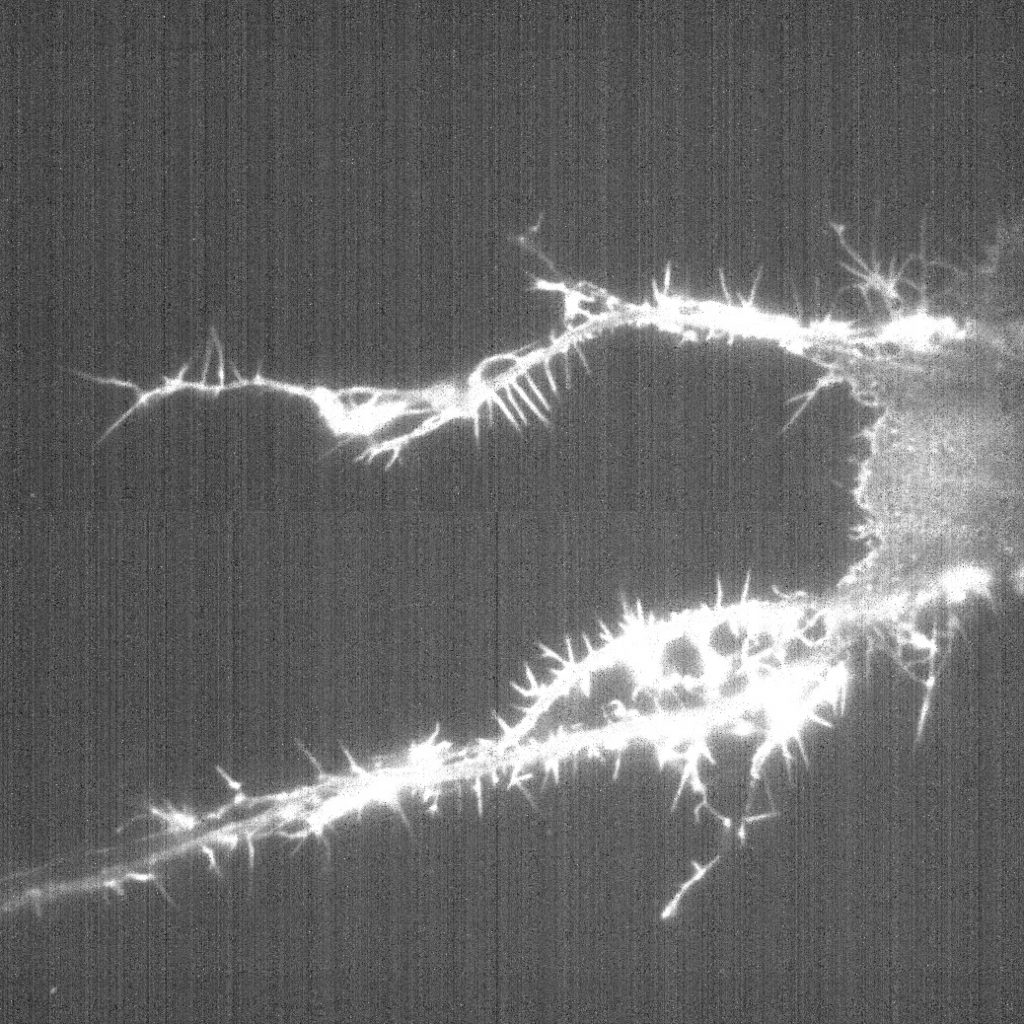
\includegraphics[width=0.6\textwidth]{images/Fixed_Noise_Pattern.jpeg}
    \caption{CMOS camera capting neurons. Average of 100 frames with 30ms exposure time. \cite{pattnoise}}
    \label{fig:fixedpatternnoise}
\end{figure}

Fixed Pattern Noise comes from two main sources: \textit{PRNU} (Photo Response Non-Uniformity) and \textit{DSNU} (Dark Signal Non-Uniformity).
Figure \ref{fig:fixedpatternnoise}] shows fixed pattern noise on the background, the column patterns are present all over the image. Frame averaging usually works to eliminate random noise, but it worsen fixed pattern noise.

PRNU is caused by responsitivity variation between pixels and it is the dominant noise in illuminated images. PRNU has a lot of properties that make it useful as an image fingerprint.
It survives lossy JPEG compression and for this reason it has been used for source identification or forgery detection. This property, however, makes PRNU bad as the basis of a PUF.
Since it survives JPEG compression, the PRNU fingerprint can be obtained by anyone, if the image is shared without proper access control (an example would be an image shared on social media).

To address this security problem, the PUF design uses DSNU fingerprint as its basis. DSNU is more difficult to be extracted in illuminated natural images, since it is not the dominant noise.

\subsection{DSNU}
\begin{figure}[h!]                      
    \centering
    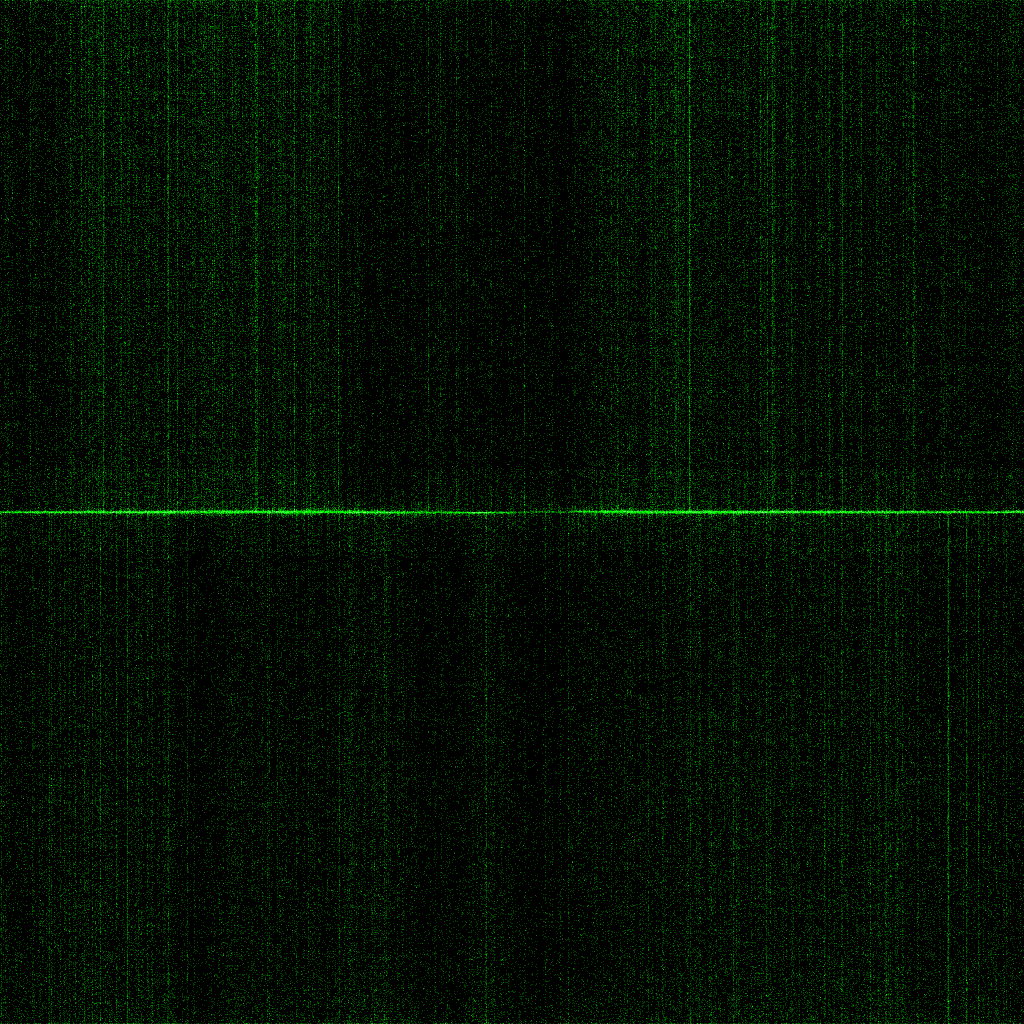
\includegraphics[width=0.6\textwidth]{images/DSNU.png}
    \caption{example of DSNU, 100 frames average with no illumination. The bias fluctuation is seen as regular column patterns. \cite{pattnoise}}
    \label{fig:dsnu}
\end{figure}

Noise in digital cameras has a fluctuating behavior, and certain random noises errors can be positive or negative, which means that with a signal of zero and some negative noise, a pixel could have a negative value.
From a software point of view, a negative value can be problematic. To avoid this, a positive offset is added to each pixel's value.

This offset creates a background effect so that, even without light, each pixel has a non-zero value, which is called \textit{bias}.
However, this bias is not constant through each pixel, because of CMOS column-to-column variations. This causes a fluctuation in the bias, which is the \textbf{DSNU}.
Figure \ref{fig:dsnu} shows DSNU on a dark image with no illumination. While illumination does not affect DSNU, temperature and exposure time does (increasing exposure causes sensor to heat).

\section{Challenge-Response Authentication}

Challenge-Response Authentication is a security protocol used to verify the identity of a user by providing a challenge, to which the user must respond correctly.
Often, the challenge would be a random nonce (random number used only once, to avoid replay attacks). The user applies a transformation on the random nonce and sends the response to the verifier.
The CamPUF design uses the DSNU fingerprint as the basis for the challenge-response authentication protocol.
This mechanism has the advantage of having a light communication overhead between the user's device and the verifier, which is useful, since CamPUF is created with low-power devices (mobile devices) in mind.

\begin{figure}[h!]                      
    \centering
    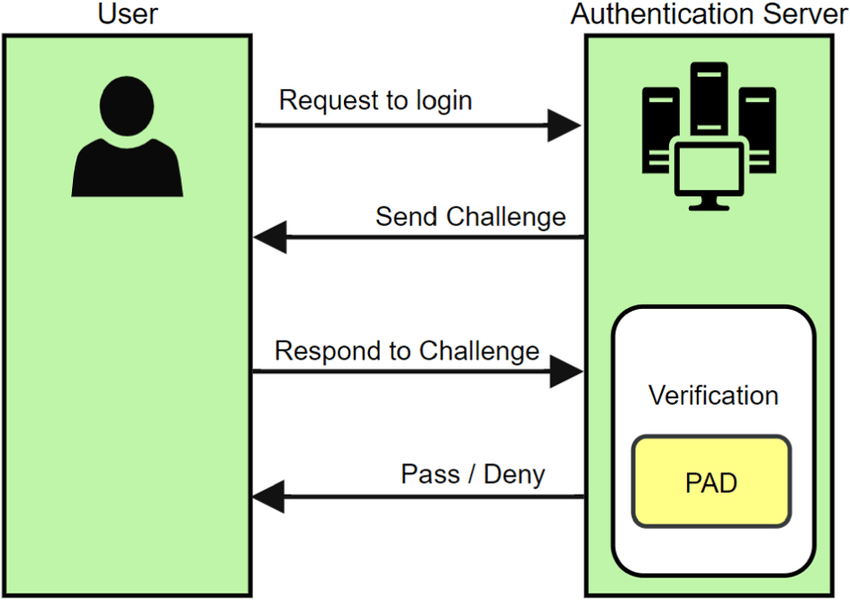
\includegraphics[width=0.6\textwidth]{images/Challenge_Response_Auth.png}
    \caption{Simple schema which shows the Challenge-Response protocol}
    \label{fig:cr_auth}
\end{figure}

The Figure \ref{fig:cr_auth} shows all the protocol steps and parties involved.

\chapter{Implementation Overview}
In this chapter you should provide a general overview of the project, explaining what you have implemented staying at a high-level of abstraction, without going too much into the details. Leave details for the implementation chapter. This chapter can be organized in sections, such as goal of the project, issues to be solved, solution overview, etc.

It is very important to add images, schemes, graphs to explain the original problem and your solution. Pictures are extremely useful to understand complex ideas that might need an entire page to be explained.

Use multiple sections to explain the starting point of your project, the last section is going to be the high-level view of your solution...so take the reader in a short `journey` to showcase your work.

\section{Introduction}
The goal of this project was to design a CMOS-based PUF on a CMOS camera-based device.
The initial phase of the project involved an extensive literature review, to explore the state of the art for CMOS-based PUFs.
After gathering documentation about various implementations, the goal was to identify a reproducible PUF design and then to implement it, using a device of our choice.

\section{Research Process}
The goal of this phase was to identify a well-documented and reproducible PUF design that could serve as a basis for our implementation.
Some material was already available through the project proposal. A comprehensive search through the internet was conducted and led to some other papers
related to PUF technologies and various PUF designs.

The usage of smartphone camera as a PUF basis is a relatively recent field, but a lot of PUF designs have been proposed. From exploiting the randomness of oxide breakdown in CMOS
sensors, to pixel variation noise. Even SRAM memory modules attached to some camera models were exploited to generate PUFs.

A particular implementation emerged as a candidate for the project. It contained a complete description of the design implementation from a mathematical point of view.
The setup used for the experiment validation was well described, together with the theory principles that were at the basis of the design.
The implementation is called CamPUF and the research paper is referenced in [?]


\section{Methodology}
Here are underlined some design choices that were made in order to adapt the implementation to suit the objectives of this project.
The source code is written in \textbf{Python}. This language seemed the optimal choice for the project. It is a general purpose programming language, one of the must popular ones
and for this reason it is rich of extensions, libraries and modules with comprehensive tools to deal with all kinds of paradigms and science fields.
Libraries such as OpenCV, scipy and numpy provided us with the tools to do signal data processing.

A particular challenge was given by the image dataset choice. The program works with RAW images to extract the pixels values. A small dataset of dark images was obtained using a medium-end digital camera (Canon EOS 750D).
A lot of problems were encountered testing this dataset, the hamming distance values with these images were very high, which means that authentication using the same dataset was unsuccessful.
Another small dataset was tested, with raw images provided by an Iphone and the same problem was encountered. 

An explanation for this behavior could be that the images were not completely dark, which means that the DSNU extraction phase captures other type of noise other than DSNU,
leading to a wrong fingerprint or sensors in modern phones could have DSNU removing capabilities, which leads to the same result: a lot of random noise on data extraction.
The choice fell on a dataset provided by the authors of the CamPUF design that used two Android phones from the last decade, plus an application developed by them which uses the Camera2 API.
The DSNU in this dataset was maximized, setting the ISO to the maximum and shutter speed set to the minimum. More information is disclosed in the \ref{sec:results} chapter.

\section{Solution Architecture}
\subsection{DSNU Fingerprint Extraction}
The first part of the implementation consists in a Signal Data Processing part, specifically the extraction of the DSNU fingerprint from a couple of frames of a dark image. 
An average of the frames is done to remove temporal noise components and a \textbf{denoising filter} is applied to eliminate noise residual.
A \textbf{DCT Filter} is also used for removing low-frequency components, so that the key generation is based only on high-frequency components, which are discarded in the JPEG compression algorithm.
This simple data processing operations are performed using the external libraries previously mentioned.

\subsection{Enrollment phase}
At this point, the device has generated its DSNU fingerprint and wants to register it to the \textit{authenticator} server.
The goal of this phase is to register the location of the brightest and darkest pixels of the high frequency component. The indices of all these locations are stored
and then sent to the authenticator.
\begin{figure}[h!]    
    \centering
    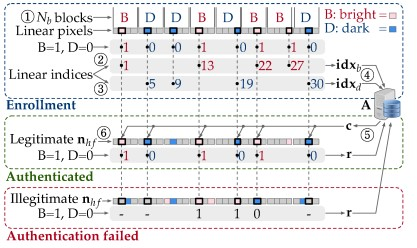
\includegraphics[width=0.5\textwidth]{images/device_auth_flow.jpg}
    \caption{Device authentication flow}
    \label{fig:authflow}
\end{figure}
\subsection{Authentication phase}
This phase is based on comparing the relative brightness of the registered pixels with the response sent from the device. The \textit{Hamming distance} is used as a
metric for measuring the similarity between the two compared keys. A threshold is selected a priori to discriminate between legitimate and illegitimate response.

Figure \ref{fig:authflow} shows the authentication flow of CamPUF.

\chapter{Implementation Details}
% This is where you explain what you have implemented and how you have implemented it. Place here all the details that you consider important, organize the chapter in sections and subsections to explain the development and your workflow.\\Given the self-explicative title of the chapter, readers usually skip it. This is ok, because this entire chapter is simply meant to describe the details of your work so that people that are very interested (such as people who have to evaluate your work or people who have to build something more complex starting from what you did) can fully understand what you developed or implemented.\\Don't worry about placing too many details in this chapter, the only essential thing is that you keep everything tidy, without mixing too much information (so make use of sections, subsections, lists, etc.). As usual, pictures are helpful.

\section{Prerequisites}\label{sec:prerequisited}
\subsection{Definitions}\label{sec:label}
The following are the elements used to explain the enrollment and authentication phase.
\begin{itemize}
  \item $L$: length of the key. 256 in the proposed implementation.
  \item $N_{m}$: noise margin.
  \item $N_{b}$: number of blocks in which the fingerprint is divided. Given by $L + N_{m}$
  \item $D$: number of pixels in the image.
\end{itemize}

\subsection{Code structure}\label{sec:projectstructure}
All the code can be found inside the \texttt{src} folder. The files are
\begin{itemize}
\item \texttt{constants.py}. The project-wide constants are set there. The \texttt{dataset\_path} variable determines which is the base directory of the dataset.
\item \texttt{extract\_dsnu.py}. The purpose of this module is providing the \texttt{get\_hf\_noise} function, which returns the fingerprint of a given image.
\item \texttt{server.py}. All the server-related operation, like the indeces registration, are implmented here.
\item \texttt{device.py}. This file exposes a function that derives the response key.
\item \texttt{auto\_testing.py}. This module is what is run
\end{itemize}

\subsection{Setup}\label{subsec:setup}
The application has been tested with Python 3.11.3 running on Arch Linux, with Linux 6.4.7.

\section{DSNU fingerprint extraction}\label{sec:dsnu_extraction}
The DSNU fingerprint extraction is implemented in the module \texttt{extract\_dsnu.py}. The only function called outside the module is \texttt{get\_hf\_noise}, while all the others are used internally.

The function \texttt{get\_hf\_noise} returns a Numpy array containing the high frequencies of the noise, and accepts as inputs a list of paths pointing to the images, width and height of the images and a boolean variable, used to determine if the resulting noise should be shown or not.

In order to obtain the fingerprint, the images are processed through the following steps.
\begin{enumerate}
\item \textbf{Calculating the average between images.}
        Before being processed, the images are opened in different ways, depending on their extension. After that, because the RAW images in the chosen dataset do not contain information about their height and width nor margins, they are reshaped using the two input parameters and the margins are cropped. In that way, a 2-D Numpy array is obtained independently the image format. This is, then, summed into an accumulator. This is sub-steps are repeated for each image in the list. Finally, when the loop ends, the average is computed, dividing the accumulator by the length of the input list.
\item \textbf{Denoising the image.}
        At this point, the average frame is denoised, invoking the \texttt{wiener} function included into \texttt{scipy.signal} module. The second parameter of the function indicates the windows dimension in which the filter is applied, $5\times5$ in this case. It should be noted that the filtering produces a floating point matrix, although before the filtering the images is an integer matrix. This is the reason of the interpolation after the filter.
\item \textbf{Retrieving the noise.}
        The noise is simply obtained subtracting the original image, with its denoised version. The function responsible of that is \texttt{absdiff} contained into the cv2 library.
\item \textbf{Removing the low frequency components.}
        In this step the unique noise pattern should be already available, but it could be also retrieved in dark images that could be shared online. Since online images are usually compressed, cutting high frequency components, only these components should be used to extract the fingerprint. Thus, a high-pass filter is applied to the noise. This is done firstly transforming it into the \emph{discrete cosine domain}, using the function \texttt{dct2}, which is a wrapper of \texttt{dct} function provided by \texttt{scipy.fftpack}, suited for a two dimensional array. Then, a filtering matrix is built. Each element $d_{i,j}$ of the matrix is defined as
        \begin{equation}
          d_{i,j} = \begin{cases} 1, & \mbox{if } i \geq H \cdot c \mbox{ and } j \geq W \cdot c\\ 0, & \mbox{otherwise} \end{cases}
        \end{equation}
        where $H$ and  $W$ are the height and the width respectively, and $c$ is the cutoff constant between 0 and 1.
        $c$ is set to $0.5$, resulting in a matrix of non-zeros values in a quarter only at the bottom-right.

        The actual filtering is realized multiplying the filtering matrix and the DCT noise by using \texttt{np.multilply}, which implements the \emph{Hadamard product}. The last step of the extraction is the the inverse of DCT operation, returning the noise to the original domain.
  \item \textbf{Plotting}
        When the function \texttt{get\_hf\_noise} is called, an additional flag \texttt{plot\_results} could be set to plot the resulting noise. If the flag is true, then three graph will show the original image, the noise of the image and the high frequency of the noise. This could be useful to check if some pattern are evident by visual inspection.

        \section{Authentication server}\label{sec:authserver}
        The server code is located in the \texttt{server.py} module. A minimal but functional server should be able of enrolling and authenticating a device.

        \subsection{Enrolling a new device}\label{subsec:enrollment}
        The enrollment operation is implemented by the function \texttt{enroll}. It requires the high frequency noise as input, as the server should not receive the RAW images. The function produces a pair of arrays, containing one the linear indeces of bright pixels and the other of dark pixels, that are used in the authentication phase to generate the challenge to send to the device requiring authentication.
        The actual indeces are computed by an auxiliary function, \texttt{get\_indeces}. This function performs the following steps. The input matrix is flattened into an array, and divided into $N_{b}$ blocks.
        It could happen that the division results into blocks of different lengths; in these cases, given $L$ the length of the array, \texttt{np.array\_split} adds an element to the first $L \% N_{b}$ elements. This detail must be considered when the linear index of a certain pixel is derived, indeed an additional $L \% N_{b}$ term must be added to each element within a block with an index bigger than the reminder itself.
        At this point, for each block the brightest pixel, corresponding to the biggest element, is found, and a new list of these pixels is built, keeping track of their block and linear index.
        Sorted the new list by brightness, from the brighter half the \texttt{idx\_bright}
        is built by means of pixels linear indeces. Finally, in the other half of the blocks, the darker pixels are sought, and, similarly to before, \texttt{idx\_dark} is built.

        \subsection{Authenticate the device}\label{sec:authdevice}
        \subparagraph{Creating the challenge.}
        When a device requires authentication, the server sends a challenge to it. The challenge depends on the previously \texttt{idx\_bright} and \texttt{idx\_dark} registered lists.
        The function that creates the challenge is \texttt{get\_challenge}. Using the function \texttt{random.sample}, $L/2$ elements are selected from \texttt{idx\_dark} and the remaining $L/2$ from \texttt{idx\_bright}. The challenge is, thus, derived merging the selected values into a single array, and then sorting it.

        \subparagraph{Checking the response.}
        After the device sends back the response key, the server must compare it with the reference key. Since the server derives at run time the key, it should be computed before. The function \texttt{get\_reference\_key} is called with the challenge and the bright indeces as parameters. It just creates a list of $0s$ and $1s$, returning a 1 if the $i$-th element of the challenge is in \texttt{idx\_bright}, otherwise a 0.
        The server function that determine if the device is authenticated is \texttt{authenticate}, that takes the reference key and the response key as inputs, and returns true or false, depending on the outcome. An additional information about the hamming distance between the two keys is returned as well, although it is more a debugging information. The function \texttt{are\_equal} computes the hamming distance and compares it with a threshold defined in \texttt{constants.py}. If the distance does not exceed the threshold, the function returns true, authenticating the device.

        \section{Device to authenticate}\label{sec:device2authenticate}
        The device produces the response key by means of the function \texttt{get\_responde\_key}. Using the fingerprint and the challenge, a list of integer is built. First of all, using the indeces in the challenge, the corresponding pixels are selected and stored in a list. Then, the median of the list is computed, and finally the response key is built. If the $i$-th element is greater than the median there is a $1$, otherwise it is a $0$.

        \section{Testing}\label{sec:testing}
        The interaction between the device and the server is tested inside \texttt{auto\_testing.py}. In this script, the fingerprint of the given image(s) path is extracted and enrolled once. Then, for each file in the authentication file list the authentication is tried, following the steps shown before.
\end{enumerate}

\chapter{Results}
% In this chapter we expect you to list and explain all the results that you have achieved. Pictures can be useful to explain the results. Think about this chapter as something similar to the demo of the oral presentation. You can also include pictures about use-cases (you can also decide to add use cases to the high level overview chapter).

\section{Testing of the CamPUF}
[TODO: write]

\subsection{Dataset}\label{sec:dataset}
After some testing, this dataset was eventually chosen \cite{dataset_url}. It is composed of various sets of both RAW and JPEG images taken with five different 12-megapixel Sony IMX377 camera sensors, used by Google Nexus 5X smartphones \cite{dataset_explanation}. The key aspect in the preference of this dataset over the others tested is that all the RAW images are completely dark photos taken with the sensor lens fully covered. This is critical since the DSNU extraction efficiency is highly influenced by the presence of any light source exposed to the sensor.

Another advantage of choosing this dataset is that it was made with the purpose of testing another CamPUF implementation, having different relevant configuration ready to test, as for images taken in different room temperatures ($25^{\circ}$C, $35^{\circ}$C and $45^{\circ}$C). It is worth noting that for any real-world practical implementation, the images provided to the enrollment/authentication algorithm should be taken in a similar way, in RAW format and trying to cover the sensor lens as much as possible.

[TODO: referring to pictures below explain why newer sensor models could have less DSNU noise to rely on]

\begin{figure}[h!]
	\vspace{0.5cm}
	\includegraphics[width=\textwidth, height=5 cm]{example-image-a}
	\caption{This is the image \emph{caption}.}
	\label{fig:dataset}
\end{figure} 

\begin{figure}[h!]
	\vspace{0.5cm}
	\includegraphics[width=\textwidth, height=5 cm]{example-image-a}
	\caption{This is the image \emph{caption}.}
	\label{fig:dataset2}
\end{figure} 

\subsection{Setup}
The dataset was then thoroughly tested using a python script \emph{auto\_testing.py} that automated the following steps:

\begin{enumerate}
	\item Reading one or multiple images (and in this case, making the pixel-wide average).
	\item Obtaining the reference key after enrolling with that image.
	\item Trying to authenticate with a set of images, one after the other, by comparing the response key with the reference key generated from the previous step. If the Hamming Distance of the two keys is below a certain threshold, then the couple (\emph{enrollment image}, \emph{authentication image}) is said to be authenticated.
	\item After trying all the images combinations, the script computes the Hamming Distance average for the couple (\emph{enrollment image}, \emph{authentication set}).
\end{enumerate}

The main difference when picking the \emph{authentication set} to use is the source sensor of the images with respect to the source sensor of the \emph{enrollment image}. Two different cases are distinguished:

\begin{itemize}
	\item \textbf{Intra-Sensor} testing: both the \emph{enrollment image} and the \emph{authentication set} come from the same source sensor.
	\item \textbf{Inter-Sensor} testing: The \emph{enrollment image} and the \emph{authentication set} come from a different sensor.
\end{itemize}

\subsubsection{Parameters}
The main parameters used were generally:
\begin{itemize}
	\item \textbf{Key Length}: 256 bits, both for the reference key and the response key.
	\item \textbf{Hamming Distance Threshold}: 4 bits.
	\item \textbf{Number of Frames Averaged}: 5 frames for the enrollment, 1 frame for the authentication.
	\item \textbf{Number of Images tested for Authentication}: generally 50 for each run, 20 in the case of temperature testing. \ref{sec:temperature}
\end{itemize}

\subsubsection{Expected Results}

For the algorithm to be of any use, when testing \textbf{Intra-Sensor} couples it is expected to yield positive results on the authentication, meaning that the \emph{Intra-Sensor Hamming Distance} between the reference key and the response key must be low enough, ideally zero. This is needed in order to avoid any false negatives where devices are incorrectly unauthorized.

Another crucial assumption is related to the opposite case, where \textbf{Inter-Sensor} couples are expected to yield negative results on the authentication, meaning that the \emph{Inter-Sensor Hamming Distance} between the reference key and the response key must be high enough, in this case ideally around 50\% of the key length to match the expected Hamming Distance of two random bit sequences. Finally, this is also needed to avoid any false positives where devices are incorrectly authorized.

\subsection{Results}
The results were gathered after several runs of the \emph{auto\_testing.py} script. The results obtained from the testing process are in line with the expected outcomes, validating the effectiveness of the CamPUF implementation. The graph below presents the Hamming Distance percentages for different scenarios, considering 1 frame and 5 frames for both \textbf{Intra-Sensor} and \textbf{Inter-Sensor} testings:

\begin{figure}[h!]
	\centering
	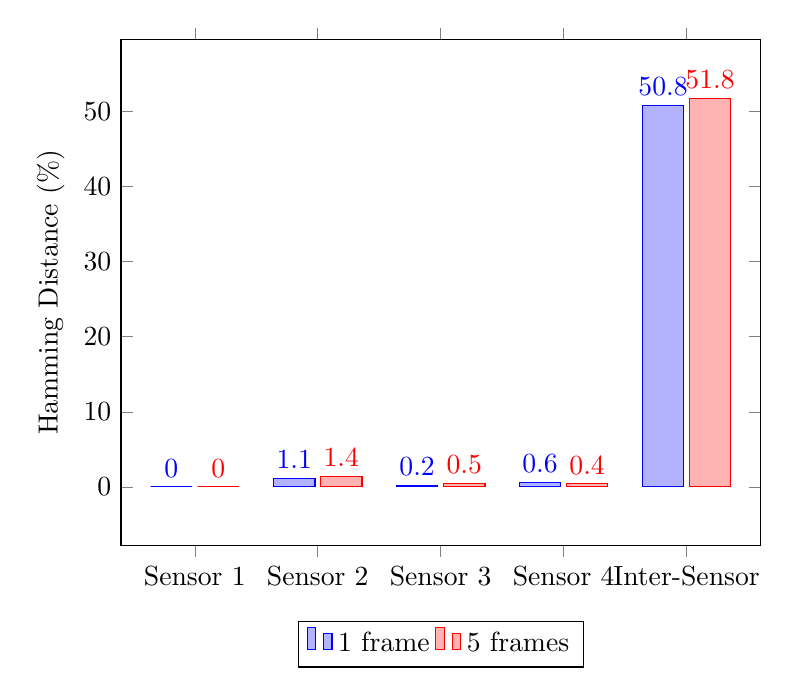
\begin{tikzpicture}
		\begin{axis}[
			width=0.8\textwidth,
			height=8cm,
			bar width=15pt,
			ybar,
			enlargelimits=0.15,
			legend style={at={(0.5,-0.15)},
			anchor=north,legend columns=-1},
			ylabel={Hamming Distance (\%)},
			symbolic x coords={Sensor 1, Sensor 2, Sensor 3, Sensor 4, Inter-Sensor},
			xtick=data,
			nodes near coords,
			nodes near coords align={vertical},
			]
			\addplot coordinates {(Sensor 1, 0.0) (Sensor 2, 1.1) (Sensor 3, 0.2) (Sensor 4, 0.6) (Inter-Sensor, 50.8)};
			\addplot coordinates {(Sensor 1, 0.0) (Sensor 2, 1.4) (Sensor 3, 0.5) (Sensor 4, 0.4) (Inter-Sensor, 51.8)};
			\legend{1 frame, 5 frames}
		\end{axis}
	\end{tikzpicture}
	\caption{Hamming Distance Percentages for Intra-Sensor and Inter-Sensor Testings}
	\label{fig:results_graph}
\end{figure}

As evident from the graph, the CamPUF algorithm performed exceptionally well in \textbf{Intra-Sensor} testing. Even with just one image for enrollment, the Hamming Distance between the reference key and the response key was found to be remarkably low. This demonstrates that a single image is sufficient to achieve accurate intra-sensor authentication, showcasing the efficiency of the algorithm.

Moreover, it was observed that a relatively low threshold of 4 bits is adequate to determine authentication success. This means that if the Hamming Distance falls below the threshold, the authentication process is successful. Fine-tuning this threshold allows for balancing between security and convenience. Lowering the threshold can increase security but may require more attempts to successfully authenticate. Conversely, increasing the threshold may reduce security but lead to faster and easier authentication.

The \textbf{Inter-Sensor} testing results align with expectations, showing Hamming Distances around 50\%, which is in line with the expected Hamming Distance between two random bit sequences. This confirms that CamPUF effectively discriminates between images taken from different sensors, providing a reliable mechanism to prevent unauthorized access.

In conclusion, the testing results demonstrate that the CamPUF implementation is capable of providing robust and accurate authentication.

\subsubsection{Temperature Resilience}

One critical aspect of the CamPUF implementation is its resilience to changes in temperature, which can impact the quality of sensor outputs. Higher temperatures often lead to increased random noise coming from the electrons inside the CMOS sensors, resulting in less noticeable DSNU noise that the algorithm relies on. We conducted testing under varying temperatures to assess the algorithm's performance in such scenarios.

The sensor tested for Intra-Sensor testing was Sensor 1, and the temperature changes refer to the room temperature relative to the images used for the authentication phase. The enrollment was always done with a room temperature of 25°C.

\begin{figure}[h!]
	\centering
	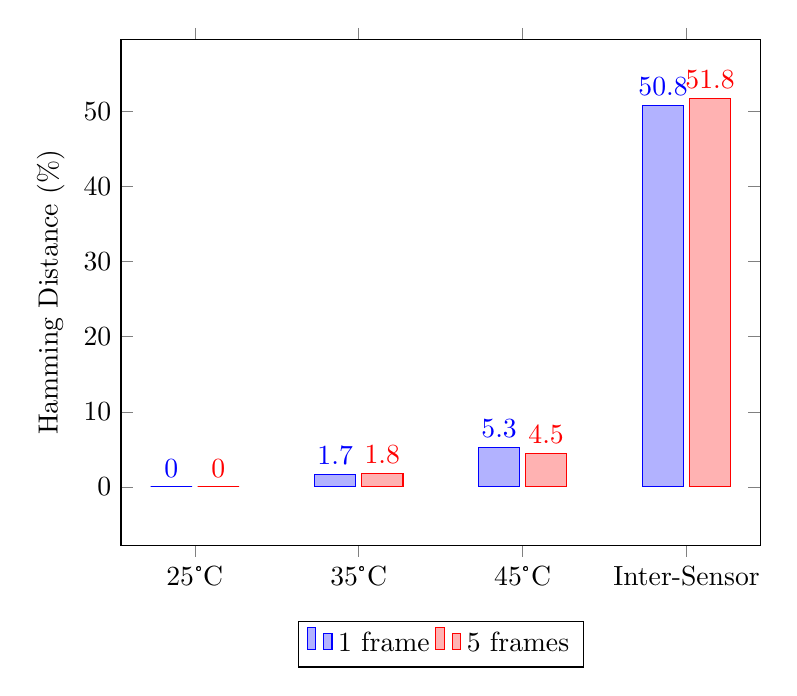
\begin{tikzpicture}
		\begin{axis}[
			width=0.8\textwidth,
			height=8cm,
			bar width=15pt,
			ybar,
			enlargelimits=0.15,
			legend style={at={(0.5,-0.15)},
			anchor=north,legend columns=-1},
			ylabel={Hamming Distance (\%)},
			symbolic x coords={25°C, 35°C, 45°C, Inter-Sensor},
			xtick=data,
			nodes near coords,
			nodes near coords align={vertical},
			]
			\addplot coordinates {(25°C, 0.0) (35°C, 1.7) (45°C, 5.3) (Inter-Sensor, 50.8)};
			\addplot coordinates {(25°C, 0.0) (35°C, 1.8) (45°C, 4.5) (Inter-Sensor, 51.8)};
			\legend{1 frame, 5 frames}
		\end{axis}
	\end{tikzpicture}
	\caption{Hamming Distance Percentages for Intra-Sensor and Inter-Sensor Testings at Different Temperatures}
	\label{fig:temperature_graph}
\end{figure}

As expected, the results show that the average Intra-Sensor Hamming Distance rises with increasing temperatures. At 25°C, the Hamming Distances remain negligible (0.0\%) for both one frame and five frames enrollments, indicating that even with minimal data, the algorithm achieves accurate authentication. However, at higher temperatures of 35°C and 45°C, the Intra-Sensor Hamming Distances slightly increase to 1.7\% and 5.3\% (for one frame enrollment), and 1.8\% and 4.5\% (for five frames enrollment), respectively.

Despite the slight increase in Intra-Sensor Hamming Distances with rising temperatures, they remain significantly low compared to the Inter-Sensor Hamming Distances, which are consistently around 50.8\% for one frame enrollment and 51.8\% for five frames enrollment. This highlights the algorithm's robustness and its ability to maintain reliable authentication even under varying temperatures.

In conclusion, the CamPUF implementation demonstrates promising temperature resilience. While the average Intra-Sensor Hamming Distance increases with higher temperatures, it remains negligible compared to the Inter-Sensor Hamming Distance. This reinforces the algorithm's effectiveness in providing secure and accurate device authentication across different environmental conditions.

\subsection{Attacks Mitigation}
TODO:

\section{Known Issues}
% If there is any known issue, limitation, error, problem, etc...explain it in this section. Use a specific subsection for each known issue. Issues can be related to many things, including design issues.
The main limitation of this implementation of CamPUF is the need for a dataset of images highly similar to the one used for testing described in \ref{sec:dataset}. Even if the TODO:


\section{Future Work}
% Adding a section about how to improve the project is not mandatory but it is useful to show that you actually understood the topics of the project and have ideas for improvements.
\label{sec:future_work}


\chapter{Conclusions}
This final chapter is used to recap what you did in the project. No detail, just a high-level summary of your project (1 page or a bit less is usually enough, but it depends on the specific project).
\begin{thebibliography}{9}
% The bibligraphy is mandatory. Here you have a couple of examples (remember to put references in the text).

\bibitem{pufwiki}
Wikipedia, \emph{Types of Physical Unclonable Functions}. \url{https://en.wikipedia.org/wiki/Types_of_physical_unclonable_function}

\bibitem{pattnoise}
Teledyne Photometrics, \emph{Pattern Noise: DSNU and PRNU}. \url{https://www.photometrics.com/learn/advanced-imaging/pattern-noise-dsnu-and-prnu}

\bibitem{oxidecmosPUF}
Chuang, K.H.; Bury, E.; Degraeve, R.; Kaczer, B.; Groeseneken, G.; Verbauwhede, I.; Linten, D. Physically unclonable function
using CMOS breakdown position. In Proceedings of the IEEE International Reliability Physics Symposium (IRPS), Monterey, CA,
USA, 2-6 April 2017; p. 4C-1.

\bibitem{pixelvarPUF}
Okura, S.; Nakura, Y.; Shirahata, M.; Shiozaki, M.; Kubota, T.; Ishikawa, K.; Takayanagi, I.; Fujino, T. P01 A Proposal of PUF
Utilizing Pixel Variations in the CMOS Image Sensor

\bibitem{SRAMPUF}
Arjona, R.; Prada-Delgado, M.A.; Arcenegui, J.; Baturone, I. Using Physical Unclonable Functions for Internet-of-Thing Security
Cameras. In Interoperability, Safety and Security in IoT; Springer: Berlin/Heidelberg, Germany, 2017; pp. 144-153.

\bibitem{campuf}
Kim Younghyun, Lee Yongwoo (2018) \emph{CamPUF: Physically Unclonable Function based on CMOS Image Sensor Fixed Pattern Noise}, IEEE Design Automation Conference 2018.

\bibitem{dataset}
Kim Younghyun, Lee Yongwoo (2018) \emph{CamPUF Dataset}, \url{https://wisest.ece.wisc.edu/research-old/mobile-and-embedded-security/campuf-dataset/}.

\bibitem{temperature}
Kenji Irie, Alan E. McKinnon, Keith Unsworth, Ian Woodhead, (2009) \emph{Measured effects of temperature on illumination-independent camera noise}, IEEE.

\bibitem{jpeg}
Marina Gardella, Tina Nikoukhah, Yanhao Li, Quentin Bammey, (2022) \emph{The Impact of JPEG Compression on Prior Image Noise}.  IEEE International Conference on Acoustics, Speech and Signal Processing (ICASSP 2022), May 2022, Singapore. pp.2689-2693.

\end{thebibliography}

%%%%%%%%%%%%%%%%%%%%%%%%%%%%%%%%%%%%%%%%%%%%%%%%%%%%%
    
% HERE IS WHERE YOU INCLUDE YOUR APPENDICES (IF ANY)

\appendix
\chapter{User Manual}
\label{usermanual}
In the user manual you should explain, step-by-step, how to reproduce the demo that you showed in the oral presentation or the results you mentioned in the previous chapters.\\ If it is necessary to install some toolchain that is already well described in the original documentation (i.e., Espressif's toolchain for ESP32 boards or the SEcube toolchain) just insert a reference to the original documentation (and remember to clearly specify which version of the original documentation must be used). There is no need to copy and paste step-by-step guides that are already well-written and available.\\The user manual must explain how to re-create what you did in the project, no matter if it is low-level code (i..e VHDL on SEcube's FPGA), high-level code (i.e., a GUI) or something more heterogeneous (i.e. a bunch of ESP32 or Raspberry Pi communicating among them and interacting with other devices).  

\input{appendices/API.tex}

%%%%%%%%%%%%%%%%%%%%%%%%%%%%%%%%%%%%%%%%%%%%%%%%%%%%%

\end{document}
